\section*{1}
\subsection*{a}
The partition function is
\eq{
Z &= \br{2\pi\h}^{-3}\int_{\mathbb{R}^3}\int_{\mathbb{R}^3}\ex{-\beta \br{\frac{|\vec{p}|^2}{2m}+\frac{k}{2}|\vec{x}|^2}}dp^3dx^3\\
&=\br{2\pi\h}^{-3}\prod_{i}\int_{\mathbb{R}}\ex{-\beta \frac{p_i^2}{2m}}dp_i\prod_{i}\int_{\mathbb{R}}\ex{-\beta \frac{kx_i^2}{2}}dx_i\\
&=\br{2\pi\h}^{-3}\br{\prod_i\sqrt{\frac{\pi 2m}{\beta}}}\br{\prod_i\sqrt{\frac{\pi 2}{\beta k}}}\\
&=\br{2\pi\h}^{-3}\br{\frac{4\pi^2m}{\beta^2 k}}^\frac{3}{2}\\
&= \br{\frac{m}{\beta^2 k \hbar^2}}^\frac{3}{2}
}
We can now calculate the internal energy
\eq{
    \braket{E} &=-\partial_\beta\ln(Z)\\
    &= -\n{3|2}\partial_\beta\ln{\frac{m}{\beta^2k\h^2}}\\
    &= -\n{3|2}\partial_\beta\br{\ln{m}-\ln{\beta^2k\h}}\\
    &= -\n{3|2}\partial_\beta\br{\ln{m}-2\ln{\beta}-\ln{k}-\ln{\h}}\\
    &= 3\partial_\beta \ln{\beta}\\
    &= \frac{3}{\beta}\\
    &= 3k_bT
}
The heat capacity is then
\eq{
C &= \partial_T \braket{E}\\
&=\partial_T\br{3k_BT}\\
&= 3k_B
}
If we consider $N$ independent atoms then the partition function is
\eq{
Z&=\frac{1}{N!h^{3N}}\int_{\mathbb{R}^3}\int_{\mathbb{R}^3}\ex{-\beta H}dp^3dx^3\\
&=\frac{Z_{sing}^N}{N!}
}
The internal energy is then
\eq{
\braket{E}&=-\partial_\beta\ln(Z)\\
&=-\partial_\beta\br{N\ln{Z_{sing}}-\ln{N!}}\\
&=-N\partial_\beta\ln{Z_{sing}}\\
&= 3Nk_BT
}
The heat capacity per particle is then
\eq{
C &= \partial_T\braket{E}\\
&=3Nk_B\\
\frac{C}{N} &= 3k_B
}
This result is in line with the Dulont-Petit law as expected.
\subsection*{b}
The partition function for a 3D quantum harmonic oscillator is
\eq{
Z_{sing}&= \sum_j\ex{-\beta E_j}\\
&=\sum_{n_x,n_y,n_z \geq 0}\ex{-\beta E_{n_x,n_y,n_z}}\\
&= \br{Z_{1D}}^3\\
&= \br{2\sinh\br{\frac{\beta\h\w}{2}}}^{-3}
}
So the total partition function for $N$ particles is then
\eq{
Z&=\frac{1}{N!}\br{2\sinh\br{\frac{\beta\h\w}{2}}}^{-3N}
}
The internal energy is
\eq{
\braket{E}&= -\partial_\beta\ln\br{Z}\\
&=-\partial_\beta\br{-3N\ln\br{\sinh\br{\frac{\beta\h\w}{2}}}+\ln\br{\frac{2^{-3N}}{N!}}}\\
&=\n{3|2}N\h\w\coth\br{\frac{\beta\h\w}{2}}\\
&=\n{3|2}N\h\w\coth\br{\frac{\h\w}{2k_BT}}\\
}
The Bose-Einstein occupation factor, which describes how many bosons occupy a particular energy level, goes as
\eq{
n_B &= \frac{g_i}{\ex{\frac{\br{\epsilon_i-\mu}}{k_BT}}-1}\\
&= \frac{1}{\ex{\frac{\epsilon_i}{k_BT}}-1}
}
For an Einstein solid we assume that every oscillator has the same energy $\epsilon_i = \h\w$ and the chemical potential $\mu=0$. We also have to assume the degeneracy $g_i=1$.
% Ask Dr. G why g_i=1 (are we just looking at the degeneracy of a single particle or is this an ensemble affect?)

If we expand $\coth$ as exponentials
\eq{
\braket{E} &= \frac{3}{2}N\h\w\br{\frac{\ex{\beta\h\w}+1}{\ex{\beta\h\w}-1}}\\
&= \frac{3}{2}N\h\w\br{n_B\br{\ex{\beta\h\w}+1}}\\
&= \frac{3}{2}N\h\w\br{n_B\br{n_B^{-1}+2}}\\
&= \frac{3}{2}N\h\w\br{2n_B+1}\\
&=3N\h\w\br{n_B+\frac{1}{2}}
}
The heat capacity follows as
\eq{
C&=\partial_T\braket{E}\\
&=\n{3|2}N\h\w\partial_T\coth\br{\frac{\h\w}{2k_BT}}\\
&=\n{3|4}N\frac{\br{\h\w}^2}{k_B}\frac{1}{T^2}\br{\coth^2\br{\frac{\h\w}{2k_B}\frac{1}{T}}-1}
}
Taking the high temperature limit for the energy
\eq{
\lim_{T \gg \frac{\h\w}{k_B}} \braket{E} & = \n{3|2}N\h\w \lim_{T \gg \frac{\h\w}{k_B}} \coth\br{\frac{\h\w}{2k_BT}}\\
}
For $0<|\gamma| < \pi $ we can Taylor expand $\coth(\gamma)$ as\footnote{We can't literally take the limit $T\rightarrow\infty$ since $\coth(\gamma)$ does not converge at $0$; but we can assume that $\frac{\h\w}{k_B}\ll T \in \mathbb{R}$}
\eq{
\coth(\gamma)\approx\frac{1}{\gamma}+\frac{\gamma}{3}-\frac{\gamma^2}{45}+\dots
}
Then to first order the energy becomes
\eq{
\braket{E} &= \frac{3}{2}N\h\w \frac{2k_BT}{\h\w}+\mathcal{O}(\frac{1}{T})\\
&\approx 3Nk_BT \textrm{ }(\textrm{for large }T)
}
The heat capacity per particle is then
\eq{
\frac{C}{N} &\approx \frac{1}{N}\partial_T(3Nk_BT)\\
&\approx 3k_B
}
Which is in-line with the Dulont-Petit law as expected.
\section*{2}
DeBye makes the following assumptions
\begin{itemize}
    \item The energy of a solid is stored in mechanical vibrations of the lattice (sound)
    \item Sound waves can be quantized and follow Bose-Einstein statistics
    \item There is a linear dispersion relationship, ie $\omega = vk$
    \item The mechanical waves have Born-Van Karman boundary conditions at the solid boundary
    \item That there are only approximately as many modes as there are atoms in our solid
    \item The mechanical modes preferred by our system are the low-energy modes centered around $k=0$
\end{itemize}
For the purposes of our calculation we make the following assumptions\footnote{I'm not following Simon's derivation because the $\frac{1}{2}$ is irritating.}
\begin{itemize}
    \item The velocity of sound is independent of polarization of the sound wave
    \item The velocity of sound is independent of the direction of propagation
    \item Our solid has even side lengths $L$
\end{itemize}
The solution to the classical 3D wave equation is as follows
\eq{
\psi(\vec{x},t) &= A\sin\br{\vec{k}\cdot \vec{x}-v|\vec{k}|t}
}
We know that $E=\hbar \w = \h v |\vec{k}|$, so summing over every mode and polarization and weighting each mode by it's occupation, we get
\eq{
\braket{E} &= 3 \sum_k\hbar v k n_B\\
&=3\br{\frac{L}{2\pi}}^3\int \hbar v k n_B d\vec{k}\\
&= 3\br{\frac{L}{2\pi}}^3\h v\int_0^{2\pi}d\phi\int_0^{\frac{1}{2}} d\theta\int_0^{k_{max}} k^3 n_B dk\\
&= 3\br{\frac{L}{2\pi}}^3\br{\frac{4\pi\h}{v^3}}\int_0^{\w_{max}}n_B \w^3 d\w\\
&= 3\br{\frac{L}{2\pi}}^3\br{\frac{4\pi\h}{v^3}}\int_0^{\w_{max}}\frac{\w^3}{\ex{\beta \w \h}-1}d\w\\
&= 3\br{\frac{L}{2\pi}}^3\br{\frac{4\pi\h}{v^3}}\br{\beta \h}^4\int_0^{x_{max}}\frac{x^3}{\ex{x}-1}dx\\
}
Where I used the DeBye sum to integral approximation, integrating over a sphere in k-space\footnote{I neglected to start with the term $\frac{1}{2}$, Simon is the only author of the the 3 others I looked at that does it this way, I'm not sure why.}.
We now use the last two assumptions of DeBye to calculate $x_{max}$. The radius of a ball containing $N$ modes is
\eq{
k_{max} &= \br{\frac{3N}{4\pi}}^\frac{1}{3}\frac{2\pi}{L}\\
\w_{max} &= \br{\frac{3N}{4\pi}}^\frac{1}{3}\frac{2\pi v}{L}\\
x_{max} &= \br{\frac{3N}{4\pi}}^\frac{1}{3}\frac{2\pi \h v}{k_B T L}\\
&=\frac{T_D}{T}
}
Where I substituted $T_D$ using the definition from Simon.
The heat capacity is then
\eq{
C&= 3\br{\frac{L}{2\pi}}^3\br{\frac{4\pi\h}{v^3}}\br{\beta \h}^4\partial_T\int_0^{\frac{T_D}{T}}\frac{x^3}{\ex{x}-1}dx\\
}
Taking the limit $T \ll T_D$ yields
\eq{
C&= 3\br{\frac{L}{2\pi}}^3\br{\frac{4\pi\h}{v^3}}\br{\beta \h}^4\partial_T\int_0^{\infty}\frac{x^3}{\ex{x}-1}dx\\
&= 3\br{\frac{L}{2\pi}}^3\br{\frac{4\pi\h}{v^3}}\br{\frac{\h}{k_BT}}^4\br{\frac{\pi^4}{15}}\\
}
Taking the limit as $T \gg T_D$ yields, after Taylor expanding the denominator to first order
\eq{
C&= 3\br{\frac{L}{2\pi}}^3\br{\frac{4\pi\h}{v^3}}\br{\beta \h}^4\br{\frac{1}{3}}\partial_T\br{\frac{T_D}{T}}^3\\
&=3Nk_BT
}
Which agrees with the Dulont-Petit law.
\section*{3}
We follow our approach in problem 2 and make the same assumptions except replacing volume with k-space area and only considering 2 polarizations
\eq{
\braket{E} &= 2\sum_khvkn_B\\
&=2\br{\frac{L}{2\pi}}^2\int \h v k n_B d\vec{k}\\
&=2\br{\frac{L}{2\pi}}^2 \h v \int_0^{2\pi}d\phi\int_0^{k_{max}} k^2 n_B dk\\
&=2\br{\frac{L}{2\pi}}^2 \br{\frac{2\pi}{\beta^3\h^2v}}\int_0^{x_{max}}\frac{x^2}{\ex{x}-1}dx
}
Where
\eq{
k_{max} &= \sqrt{\frac{N}{\pi}}\frac{2\pi}{L}\\
\w_{max} &=\sqrt{\frac{N}{\pi}}\frac{2\pi}{L}v\\
x_{max} &=\sqrt{\frac{N}{\pi}}\frac{2\pi}{L}\br{\frac{v\h}{k_BT}}
}
The heat capacity is then
\eq{
C&= 2\br{\frac{L}{2\pi}}^2 \partial_T\br{\br{\frac{2\pi}{\beta^3\h^2v}}\int_0^{\sqrt{\frac{N}{\pi}}\frac{2\pi}{L}\br{\frac{v\h}{k_BT}}}\frac{x^2}{\ex{x}-1}dx}
}
In the low temperature limit $x_{max}\rightarrow \infty$ and we get
\eq{
\int_0^\infty\frac{x^2}{\ex{x}-1}dx&= \Gamma(3)\zeta(3)\\
&=2\zeta(3)
}
So the heat capacity becomes
\eq{
C&= 2\br{\frac{L}{2\pi}}^2 \partial_T\br{\br{\frac{2\pi T^3}{k_B^3\h^2v}}2\zeta(3)}\\
&= 2\br{\frac{L}{2\pi}}^2 \br{\frac{2\pi}{k_B^3\h^2v}}2\zeta(3)T^2\\
}
So it follows that
\eq{
K &= 2\br{\frac{L}{2\pi}}^2 \br{\frac{2\pi}{k_B^3\h^2v}}2\zeta(3)\\
n &= 2
}
In the high temperature limit $x$ becomes small and we can Taylor expand the denominator as before
\eq{
\int_0^\epsilon \frac{x^2}{\ex{x}-1}&\approx \int_0^\epsilon \frac{x^2}{x}dx\\
&\approx \int_0^\epsilon xdx\\
&\approx \frac{1}{2}\epsilon\\
}
The heat capacity then becomes
\eq{
C&=2\br{\frac{L}{2\pi}}^2 \partial_T\br{\br{\frac{2\pi}{\beta^3\h^2v}}\frac{1}{2}\br{\sqrt{\frac{N}{\pi}}\frac{2\pi}{L}\br{\frac{v\h}{k_BT}}}^2}\\
&=\partial_T\br{2Nk_BT}\\
&=2Nk_BT
}
\pagebreak
\section*{4}
The provided heat capacity data is plotted below. The first plot shows the heat capacity in units of $\frac{\mu J}{K mol}$ along with the heat capacity at the Dulong-Petit limit. Both of these plots were scaled to show the heat capacity per mole of material. The second plot shows the normalized heat capacity per Kelvin per temperature squared, this is so that the cubic term that contains the DeBye temperature becomes linear. The Polyfit function in MatLab was used to calculate the 3rd order term of the un-normalized heat capacity data, then this value was used to calculate $T_{DeBye}^3$.
\begin{figure}[h]
    \centering
    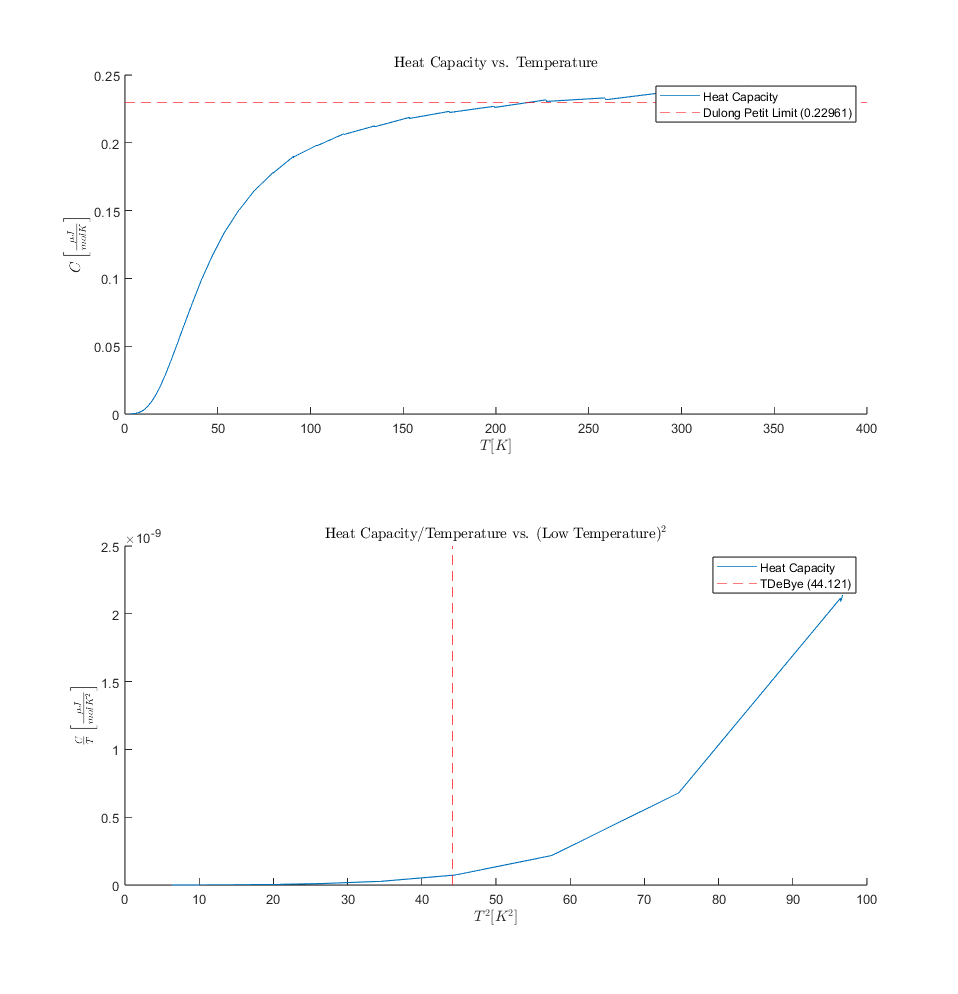
\includegraphics[width=1\linewidth]{Resources//140A//Homework 1/140A Homework 1 Problem 4.png.png}
    \caption{Heat Capacity vs. Temperature and Heat Capacity/Temperature vs Temperature$^2$.}
    \label{fig:enter-label}
\end{figure}